
\section{Motivations}
\begin{frame}

%Columns which are aligned with the first ligne for basis
\begin{columns}[t]

\begin{column}{0.375\textwidth}

\vspace{1cm}

% trim: left, bottom, right, up
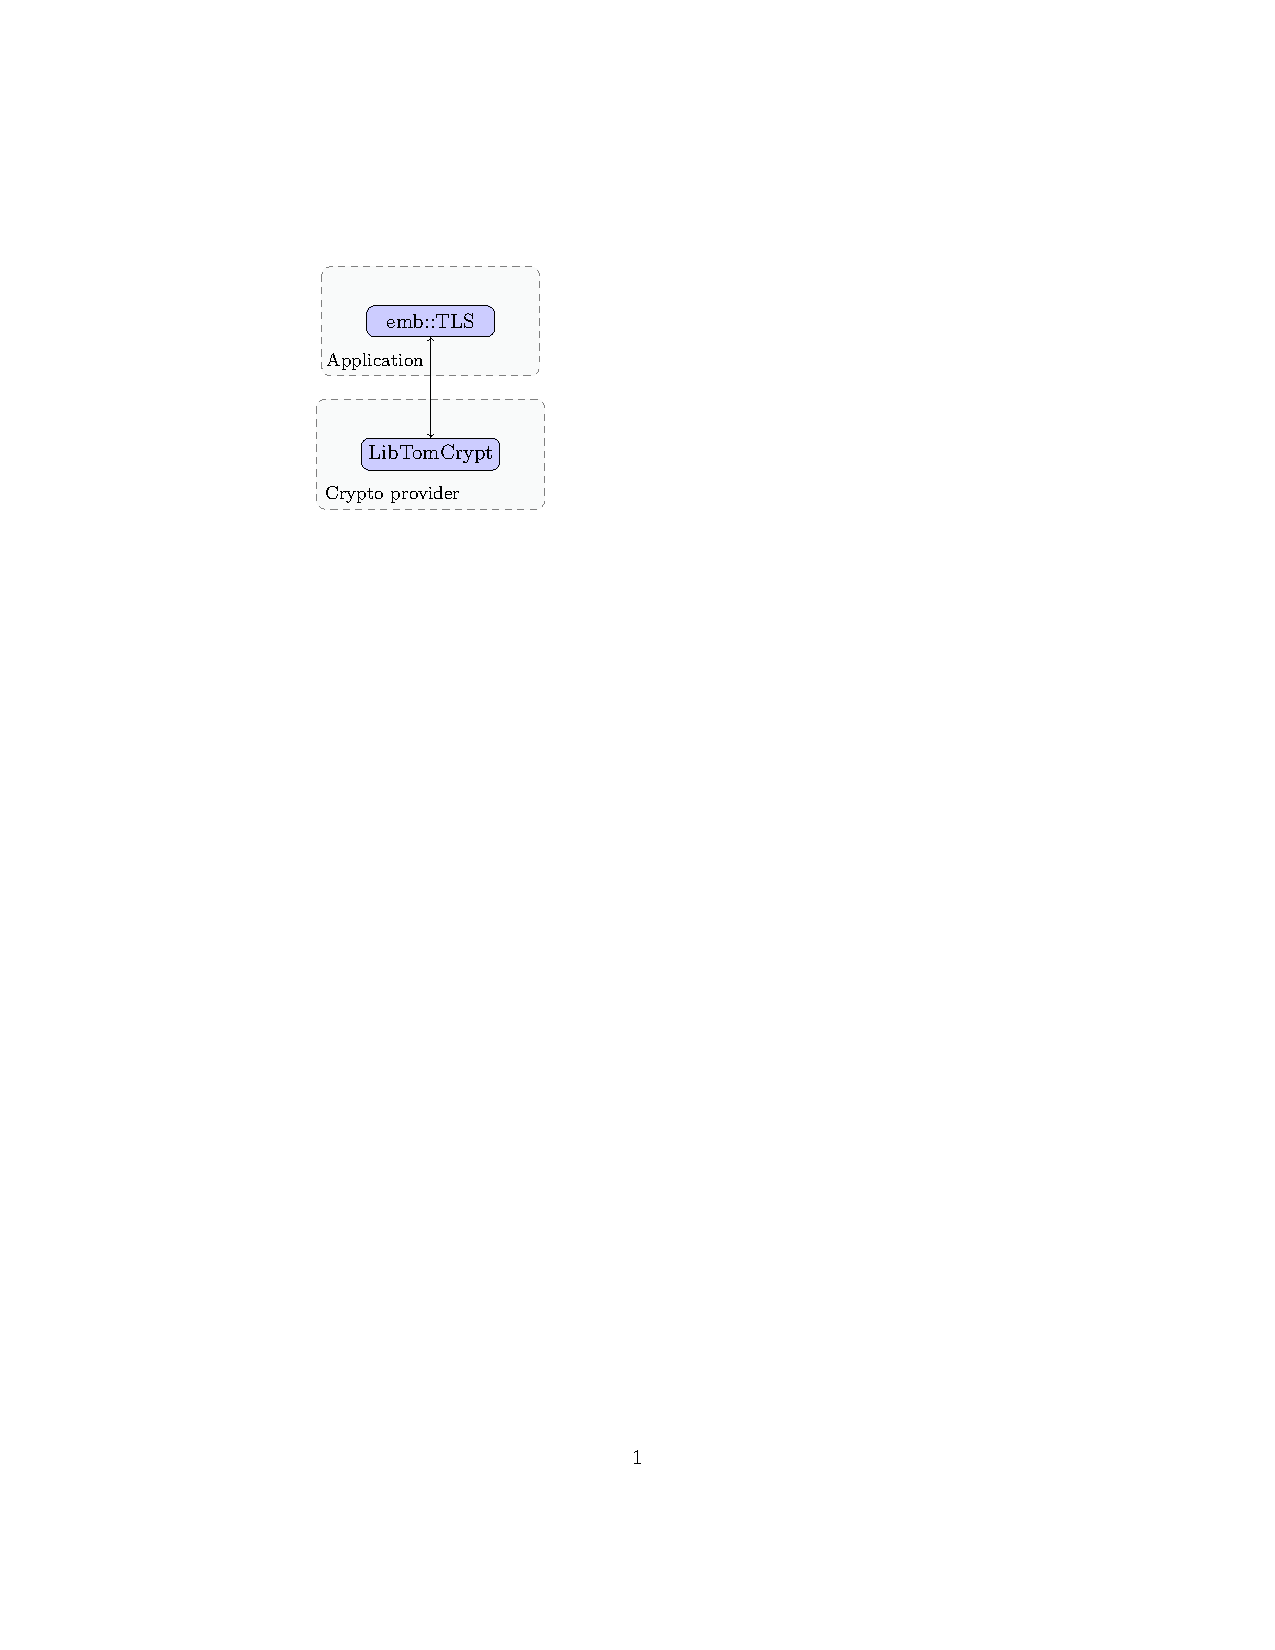
\includegraphics[trim=5cm 5cm 14cm 4.25cm]{figures/intro_cw.pdf}

\end{column}

\begin{column}{0.625\textwidth}

% trim: left, bottom, right, up
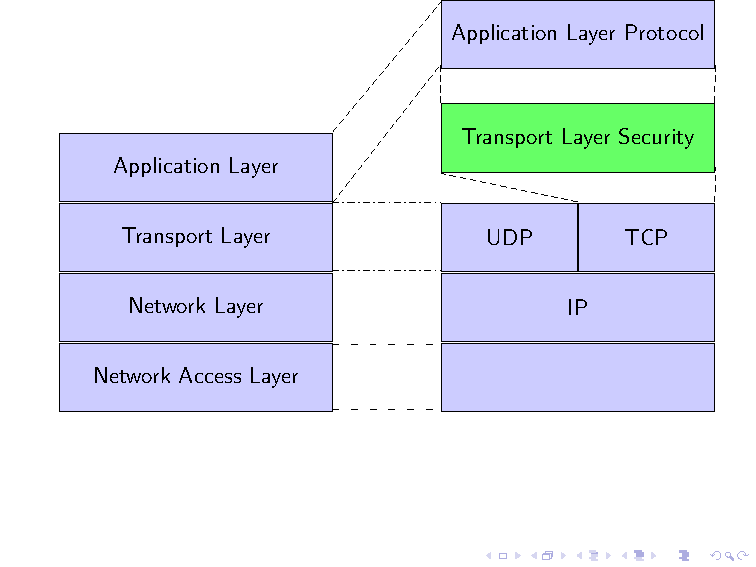
\includegraphics[trim=0cm 20cm 15cm 0cm, height=4cm]{figures/tls_osi.pdf}

\begin{itemize}
  \item  \small{\embtls}
  	\begin{itemize}
  		\item \small{Transport Layer Security (TLS) application for embedded
  		systems}
	\end{itemize}
  \item \small{\tomcrypt}
  	\begin{itemize}
  	  \item \small{open source cryptographic software library}
  	\end{itemize}
  
\end{itemize}

\end{column}

\end{columns}

\end{frame}


\begin{frame}

\begin{columns}[t]

\begin{column}{0.375\textwidth}

\vspace{1cm}

% trim: left, bottom, right, up
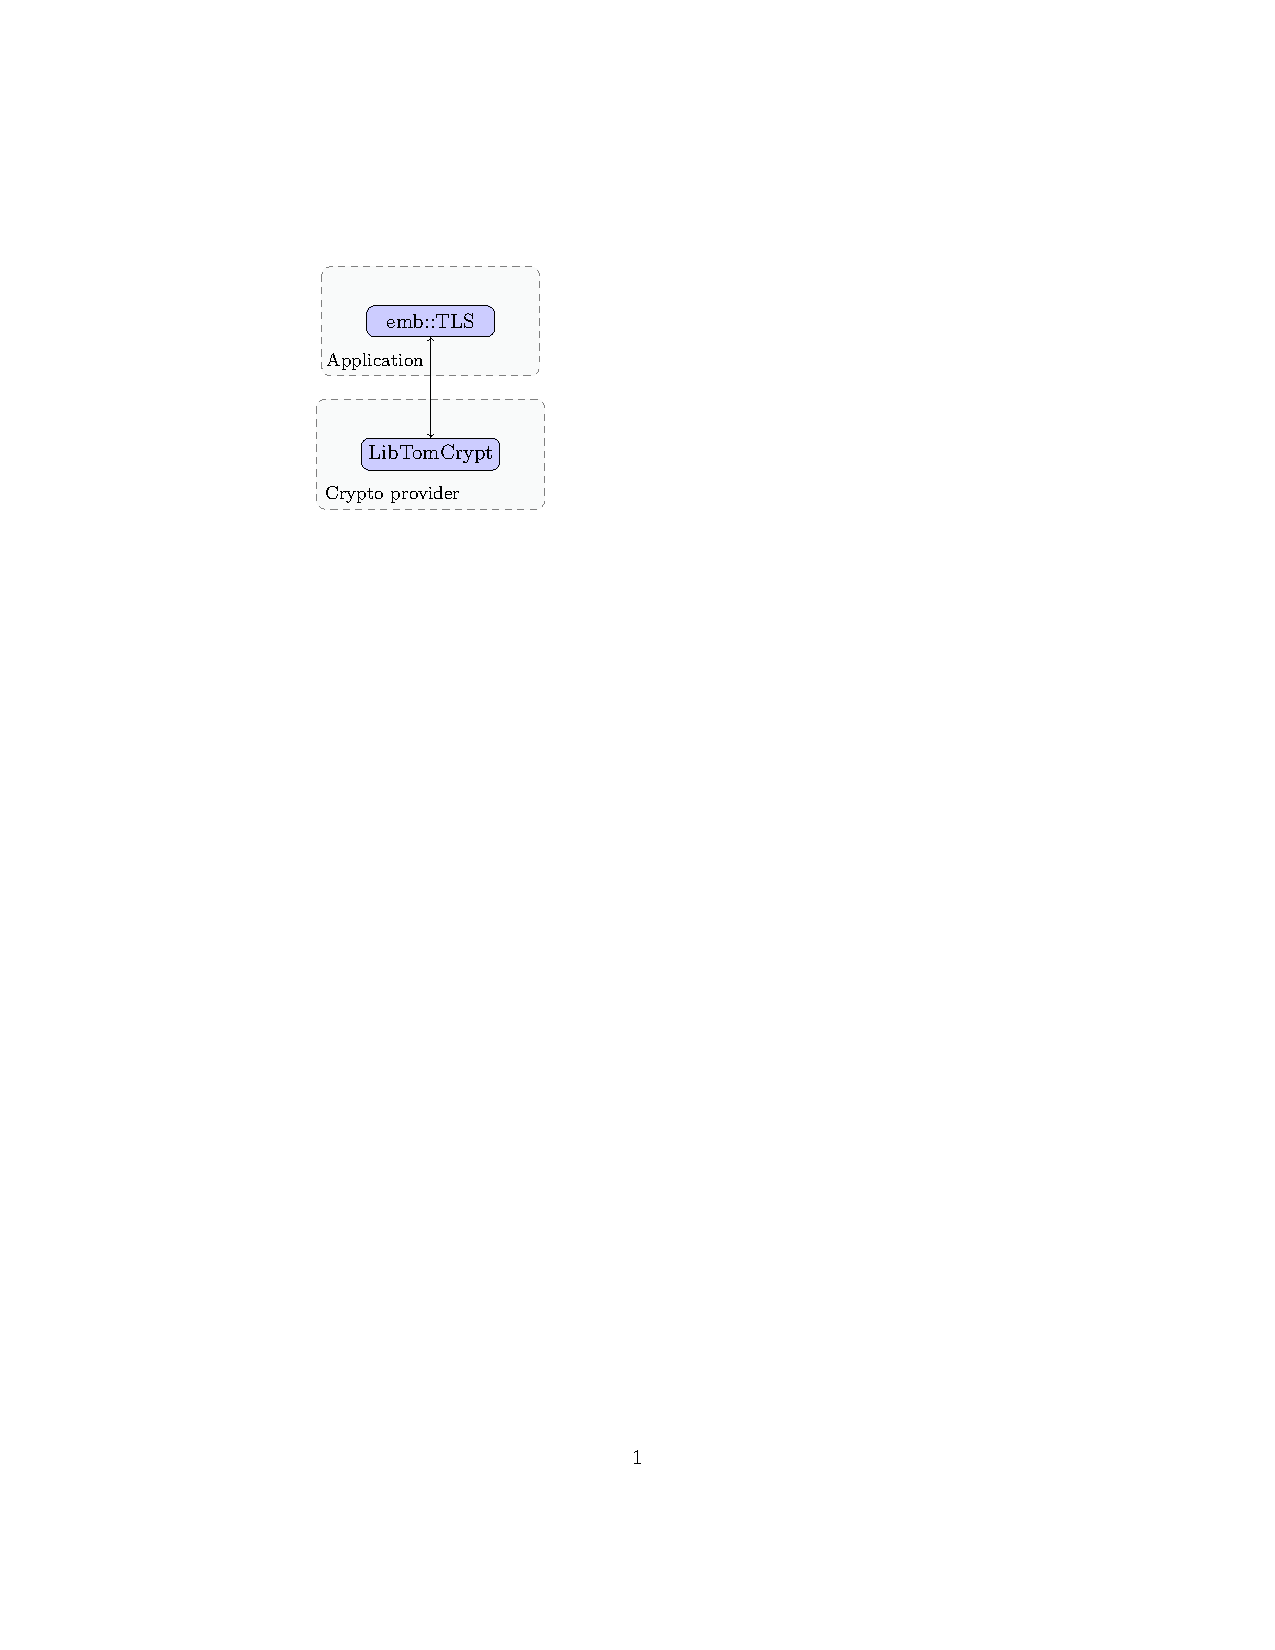
\includegraphics[trim=5cm 5cm 14cm 4.25cm]{figures/intro_cw.pdf}

\end{column}

\begin{column}{0.625\textwidth}

\vspace{1.75cm}

\underline{Requires significant manual effort}:
\begin{itemize}
  \item Only \tomcrypt is supported as cryptographic provider
  \item Many parts of the application have to be modified to use another
  provider
\end{itemize}

\end{column}

\end{columns}

\end{frame}


\begin{frame}

\begin{columns}

\begin{column}{0.475\textwidth}

\vspace{1.5cm}

%\frame{
% trim: left, bottom, right, up
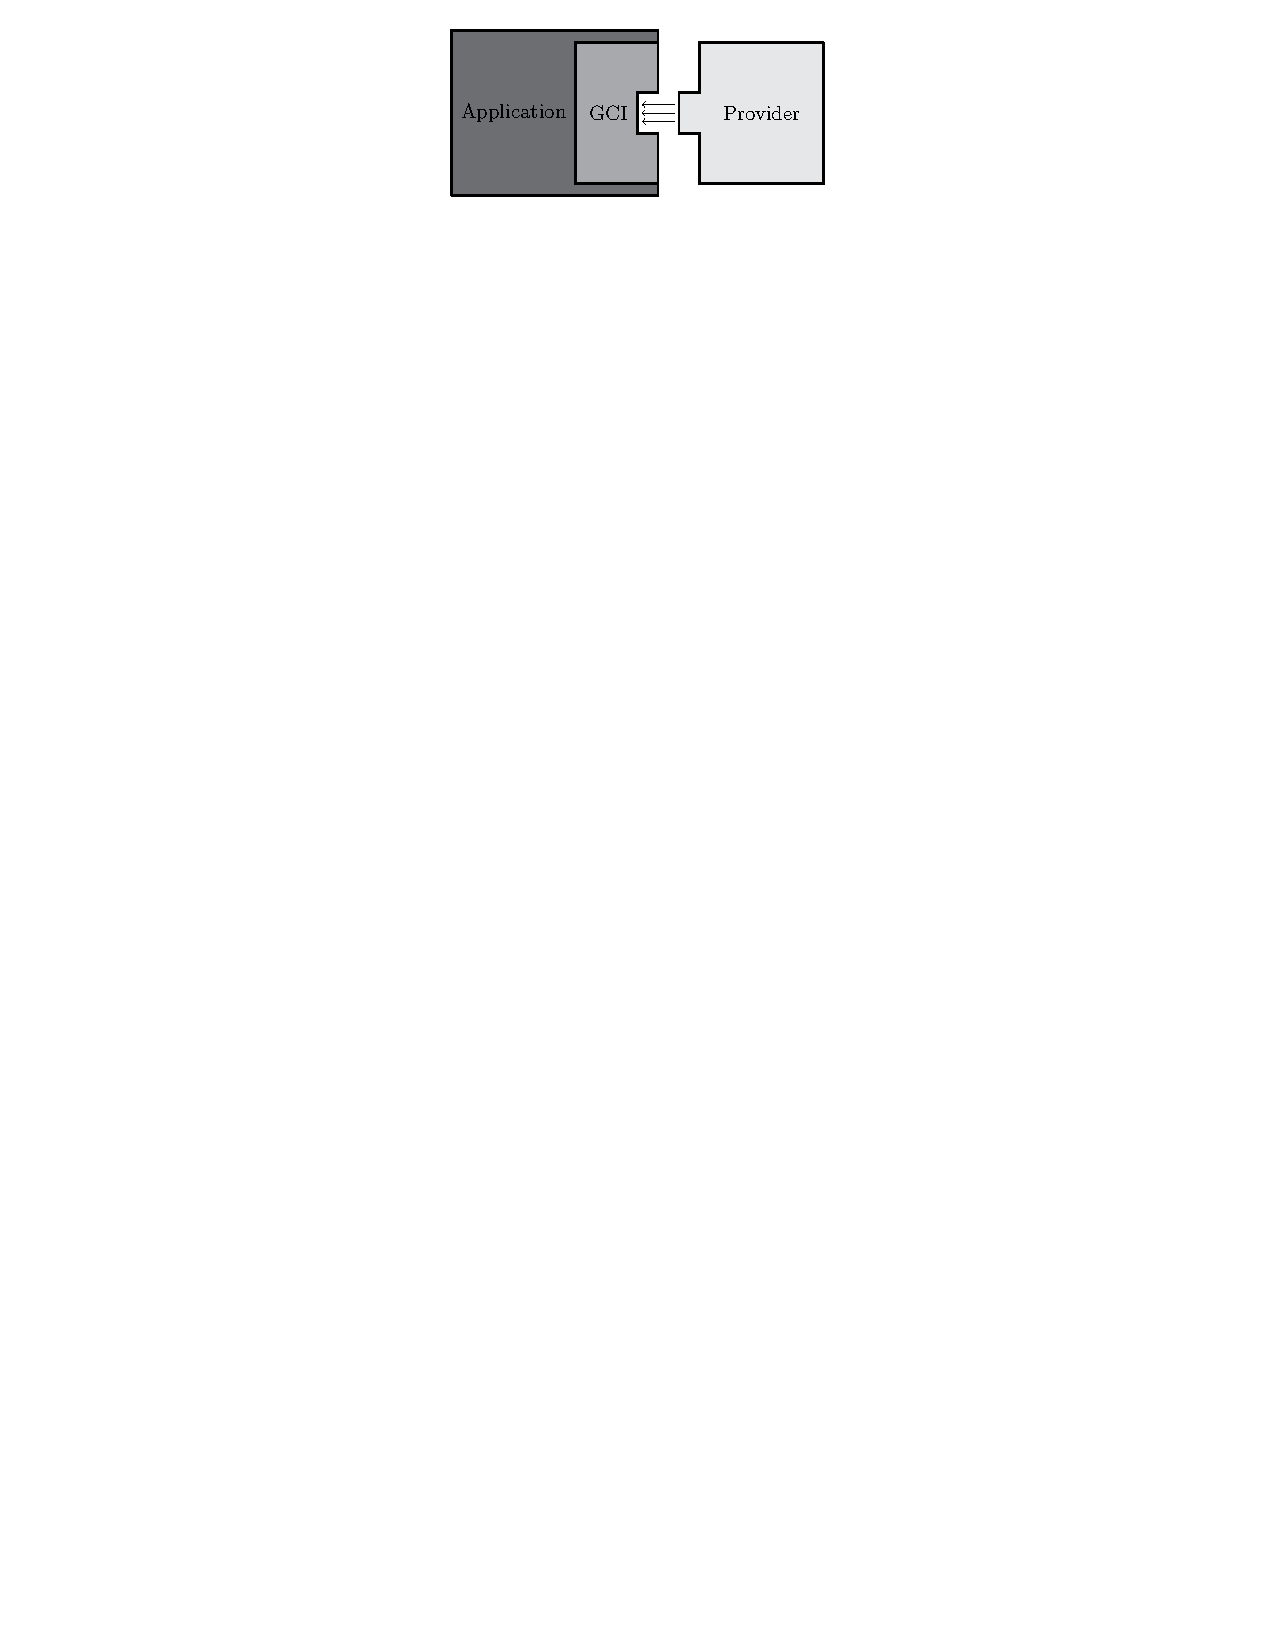
\includegraphics[trim=8cm 22cm 7cm 0cm, height=5.5cm]{figures/oli_intro.pdf}
%}
\end{column}

\begin{column}{0.525\textwidth}

\underline{Generic Cryptographic Interface (GCI)}
\begin{itemize}
  \item Provides a base of cryptography
  \item Facilitates the support of different cryptographic providers
  \item Facilitates the addition of new cryptographic algorithms

\end{itemize}

\end{column}

\end{columns}

\end{frame}




